%In de besprekeking ga ik het volgende aanhalen:
%-Aanhalen van de verschillende technologieen
%-Het onderbouwen waarom ik zo te werk ben gegaan -> hier worden de bronnen gebruikt
\chapter{Bespreking}\label{hfdst:bespreking}
In dit hoofdstuk zal de structuur die in Hoofdstuk~\vref{hfdst:situering} werd opgebouwd, verder uitgebouwd worden.
In de loop van dit hoofdstuk zullen de verschillende technologieën besproken worden die in aanmerking komen voor de verschillende componenten.
Naar het einde van het hoofdstuk toe, zal een keuze gemaakt worden en zal voor iedere component de meest geschikte technologie gekozen worden.

\section{Packager}
De eerste component die besproken wordt is de packager.
Zoals reeds besproken, moet tijdens het ontwerpen van deze component rekening gehouden worden met enkele eigenschappen.
Alvorens bepaald wordt welke technologie geschikt is, moet onderzocht worden wat ingepakt moet worden en op welke manier.

%\citet{deploymentMethods} haalt drie methodes aan om software te deployen: disk image-based deployment, behavior-based deployment en package-based deployments.
%Bij disk image-based deployment worden de software en het besturingssysteem op eenzelfde moment naar de target node verzonden.
%Er zullen verschillende image servers aanwezig zijn die elk een service aanbieden.
%Het voordeel van deze strategie is dat, zolang de hardware en software vereisten voldaan zijn, de deployment bestaat uit een simpele read-write operatie.
%Maar, zoals \citet{deploymentMethods} al aangeeft, deze methode is niet flexibel.
%Voor de applicatie is flexibiliteit een must.
%Iedere node bevat verschillende hardware en is verschillende geconfigureerd.
%Een disk image-based deployment zal hierdoor niet gebruikt worden.
%Het basis idee achter behavior-based deployment is het opnemen van de schijf operaties tijdens het deployen.
%Als geweten is welke bestanden aangepast zijn, gecreëerd zijn, ... dan kan het proces nagebootst worden op andere nodes \citep{deploymentMethods}.
%Zo een proces nabootsen is moeilijk.
%Kernel operaties moeten getraceerd worden.
%Deze methode biedt een verhoogde flexibiliteit aan ten opzichte van de disk image-based deployment maar dit is nog niet voldoende om deployments uit te voeren die uniek zijn per node.
%De laatste techniek die \citet{deploymentMethods} aan haalt is package-based deployment.
%Met behulp van een batch file, waarin alle nodige commando's aanwezig zijn, kan een installatie pakket gedeployed worden naar een target node.
%Door het gebruik van een batch file wordt de flexibiliteit van de deployment verhoogd.
%Dit is een strategie die bruikbaar is voor het probleem op te lossen.
%Voor ieder pakket kan een specifieke batch file gemaakt worden.
%Deze strategie biedt de flexibiliteit die nodig is voor het oplossen van het probleem.
%
%Om een correct werkende applicatie te hebben, heeft het Python raamwerk verschillende drivers en bibliotheken nodig.
%\citet{Obreshkov2008244} bespreekt hoe het ATLAS project te werk gaat bij het inpakken van alle nodige software.
%Het ATLAS project gebruikt CMT als configuratie manager.
%Met behulp van een configuratie bestand weten verscheidene tools hoe ze een pakket moeten afhandelen \citep{Obreshkov2008244}.
%Een gelijkaardige structuur is wenselijk voor het probleem.
%Net zoals \citet{Obreshkov2008244} zou er voor ieder bibliotheek en driver een pakket voorzien worden.
%Hierdoor wordt de herbruikbaarheid bevordert en kan voor ieder pakket apart behandelt worden.
%%%% SAUCE gebruiken om statement te ondersteunen
%\citet{packAtlas} spreekt ook over CMT als informatiebron voor het ophalen van meta-data.
%Aan de hand van deze data kan een Pacman pakket geproduceerd worden.
%Met behulp van een ``Pacman file'' is geweten hoe de ingepakte software behandelt moet worden.

%\subsection{Technologieën}
%In voorbereiding op het academiejaar, was het mogelijk om een stage te lopen bij het bedrijf.
%Het doel van deze stage was het voorbereiden van de thesis.
%Tijdens deze voorbereiding, werd er vooral gezocht naar een goede technologie die gebruikt kon worden voor de packager.
%In wat volgt, gaat er een opsomming volgen van de onderzochte technologieën samen met hun voor- en nadelen.
%
%%%% TODO schrijven van voor- en nadelen van de verschillende techs
%%%% LAYOUT paragraph of subsection?
%%%% LAYOUT 1 of meerdere tabellen?
%\subsubsection{WiX Toolset}
%Windows installer XML Toolset is een set van build tools waarmee Windows Installer packages gemaakt kunnen worden.
%Bron code wordt gecompileerd en vervolgens gelinkt om een executable te maken.
%De toolset zal .msi installatie pakketten, .msm merge modules en .msp patches combineren \citep{wixToolset}.
%
%Aan deze technologie zijn verschillende plus- en minpunten verbonden.
%Een vergelijking van de verschillende voor- en nadelen is terug te vinden in Tabel~\ref{tab:wix}.
%In de tabel wordt vermeld dat WiX een diepe integratie heeft met Windows.
%Dit komt doordat WiX installers produceert voor de Windows Installer, het Windows installation engine.
%Zulke installers worden gemaakt aan de hand van XML bestanden die de verschillende elementen definiëren  \citep{wixTutorial}.
%\citet{xmill} haalt verschillende eigenschappen aan van XML waar rekening gehouden moet worden.
%XML is niet het meest efficiënte dataformaat maar biedt een verhoogde flexibiliteit aan.
%
%\begin{table}
%\begin{tabularx}{\linewidth}{>{\parskip1ex}X@{\kern4\tabcolsep}>{\parskip1ex}X}
%\toprule
%\hfil\bfseries Voordelen
%&
%\hfil\bfseries Nadelen
%\\\cmidrule(r{3\tabcolsep}){1-1}\cmidrule(l{-\tabcolsep}){2-2}
%
%%% PROS, seperated by empty line or \par
%Diepe integratie met Windows \par
%Mogelijkheid om externe executables te includeren
%&
%%% CONS, seperated by empty line or \par
%XML structuren zorgt voor veel schrijfwerk \par
%Niet cross-platform
%\\\bottomrule
%\end{tabularx}
%\caption{Voor- en nadelen WiX Toolset}
%\label{tab:wix}
%\end{table}
%
%\subsubsection{NSIS}
%Nullsoft Scriptable Install System is een open source systeem waarmee Windows installers gemaakt kunnen worden.
%Zoals de naam aangeeft, is NSIS script-based waardoor installers logica bevatten waarmee verschillende installatie taken  behandelt kunnen worden.
%Hiernaast bestaan er al verschillende plug-ins en scripts voor verschillende taken af te handelen \citep{nsisMain}.
%
%Aan deze technologie zijn verschillende plus- en minpunten verbonden.
%Een vergelijking van de verschillende voor- en nadelen is terug te vinden in Tabel~\ref{tab:nsis}.
%Aangezien NSIS een scripting taal gebruikt om een installer te definiëren, is het zeer eenvoudig om een eenvoudige installer te creëren.
%Gecombineerd met de grote hoeveelheid aan plug-ins die aanwezig zijn door de community, wordt het eenvoudig om een installer te produceren die het probleem kan oplossen.
%De tool ondersteunt geen structuur waarmee verschillende pakketten gedefinieerd kunnen worden.
%Zoals WiX Toolset is deze technologie uitsluitend voor Windows.
%
%\begin{table}
%\begin{tabularx}{\linewidth}{>{\parskip1ex}X@{\kern4\tabcolsep}>{\parskip1ex}X}
%\toprule
%\hfil\bfseries Voordelen
%&
%\hfil\bfseries Nadelen
%\\\cmidrule(r{3\tabcolsep}){1-1}\cmidrule(l{-\tabcolsep}){2-2}
%
%%% PROS, seperated by empty line or \par
%Scripting taal \par
%Verschillende plug-ins beschikbaar
%&
%%% CONS, seperated by empty line or \par
%Niet cross-platform\par
%Geen structuur voor packages
%\\\bottomrule
%\end{tabularx}
%\caption{Voor- en nadelen NSIS}
%\label{tab:nsis}
%\end{table}
%
%\subsubsection{Chocolatey}
%Volgens \citet{chocoAbout} is Chocolatey een package mangager voor Windows net zoals apt-get voor Linux is.
%Het is ontworpen als een gedecentraliseerd framework met als doel het snel installeren van applicaties en tools.
%Het werd gebouwd boven op het NuGet infrastructuur en gebruikt PowerShell als zijn focus voor het verspreiden van de packages.
%
%Aan deze technologie zijn verschillende plus- en minpunten verbonden.
%Een vergelijking van de verschillende voor- en nadelen is terug te vinden in Tabel~\ref{tab:choco}.
%Het grootste voordeel dat bekomen wordt bij het gebruiken van een package manager is het al bestaan van een deployment infrastructuur. 
%Na het installeren van Chocolatey op de client kunnen alle nodige packages voor het framework geïnstalleerd worden.
%Hiernaast kunnen scripts gekoppeld worden aan iedere package zodanig dat een aangepaste installatie mogelijk is.
%Net zoals apt-get voor Linux, is Chocolatey te gebruiken in de command-line.
%Dit is vooral een nadeel naar gebruiksvriendelijkheid toe aangezien er vanuit wordt gegaan dat de gebruikers amper tot geen ervaring hebben met de command-line in Windows/Linux.
%Het grootste nadeel aan deze technologie is, net zoals de vorige opties, het niet cross-platform zijn.
%
%\begin{table}
%\begin{tabularx}{\linewidth}{>{\parskip1ex}X@{\kern4\tabcolsep}>{\parskip1ex}X}
%\toprule
%\hfil\bfseries Voordelen
%&
%\hfil\bfseries Nadelen
%\\\cmidrule(r{3\tabcolsep}){1-1}\cmidrule(l{-\tabcolsep}){2-2}
%
%%% PROS, seperated by empty line or \par
%Volledige deployment infrastructuur al aanwezig\par
%&
%%% CONS, seperated by empty line or \par
%Niet cross-platform\par 
%Command-line tool
%\\\bottomrule
%\end{tabularx}
%\caption{Voor- en nadelen Chocolatey}
%\label{tab:choco}
%\end{table}
%
%\subsubsection{Qt Installer Framework}
%Het Qt Installer Framework biedt een set van tools aan voor het creëren van installers op verschillende platformen.
%Aan de hand van een set van pagina's wordt de gebruiker door het installatie-, update- en verwijderproces.
%Hierbij kunnen scripts gebruikt worden om het proces te vereenvoudigen \citep{qtDoc}.
%
%Aan deze technologie zijn verschillende plus- en minpunten verbonden.
%Een vergelijking van de verschillende voor- en nadelen is terug te vinden in Tabel~\ref{tab:qt}.
%Het grootste voordeel van het Qt Installer framework is het cross-platform zijn.
%Hierdoor is het mogelijk om installers te maken voor zowel Windows als Linux.
%Een nadeel dat hieraan verbonden is, is dat een Linux installer enkel kan gemaakt worden op in een Linux omgeving.
%Het is niet mogelijk om een Linux installer te maken op een Windows systeem.
%Hiernaast is het wel mogelijk om voor ieder pakket een aparte installatieprocedure te implementeren.
%
%\begin{table}
%\begin{tabularx}{\linewidth}{>{\parskip1ex}X@{\kern4\tabcolsep}>{\parskip1ex}X}
%\toprule
%\hfil\bfseries Voordelen
%&
%\hfil\bfseries Nadelen
%\\\cmidrule(r{3\tabcolsep}){1-1}\cmidrule(l{-\tabcolsep}){2-2}
%
%%% PROS, seperated by empty line or \par
%Cross-platform \par
%Mogelijkheid om externe executables te includeren
%&
%%% CONS, seperated by empty line or \par
%XML structuren zorgt voor veel schrijfwerk \par
%Enkel Linux installer maken in Linux
%
%\\\bottomrule
%\end{tabularx}
%\caption{Voor- en nadelen Qt Installer Framework}
%\label{tab:qt}
%\end{table}
%
%%%% TODO
%Schrijven over het gebruiken van Windows .exe in Linux? Bijvoorbeeld hoe Wine misschien een oplossing is?
%
%%%% TODO
%Schrijven over de test setup voor de verschillende technologieën die gebruikt is tijdens de stage?

%%% TODO
Schrijven over waarom Qt effectief is gekozen

%\subsection{Databank}\label{sec:databank}
%Het aantal pakketten die gebruikt gaan worden, gaan alleen toenemen.
%Naast deze groei zullen ook het aantal gebruikers toenemen.
%Daarom werd er geopteerd om een databank te ontwerpen voor het opslaan van alle cruciale data.
%In overleg met het bedrijf werd ervoor gekozen om MySQL te gebruiken als managementsysteem.
%Het ontwerp van de databank is terug te vinden in Figuur~\vref{fig:databank}.
%
%\begin{figure}[!ht]
%\centering
%\makebox[0pt]{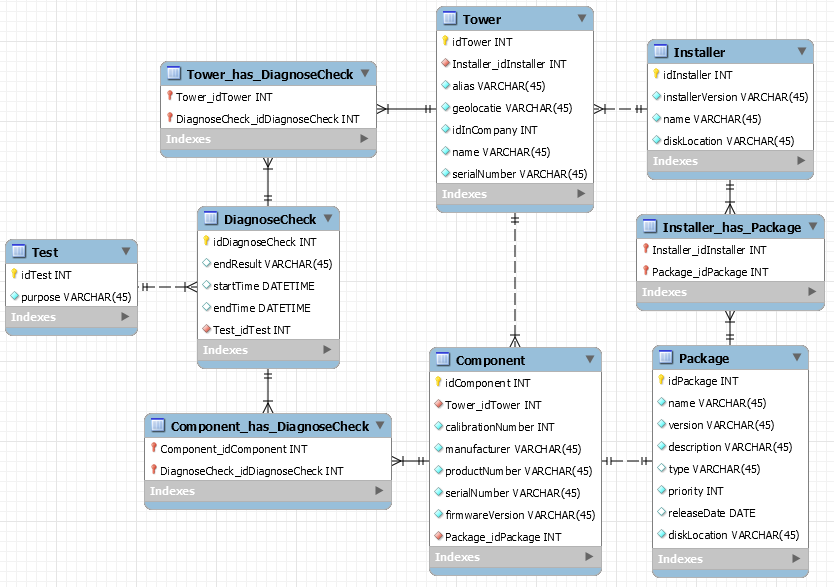
\includegraphics[scale=0.5]{afbeelding/databankOntwerp.png}}
%\caption{Ontwerp van de databank}
%\label{fig:databank}
%\end{figure}
%
%Tijdens het ontwerp van de databank, in overleg met het bedrijf, zijn er verschillende keuzes gemaakt die moeten toegelicht worden.
%Dit ontwerp weerspiegelt de structuur die aangehaald werd in Figuur~\vref{fig:overzichtsDiagram} met als verschil dat in het ontwerp de client centraal staat en niet de server.
%Verder zullen de verschillende tabellen overlopen worden en enkele termen vastgelegd worden zodanig dat deze een eenduidige betekenis gedurende de rest van de thesis.
%Centraal staan alle tabellen horende bij de een testtoren.
%Iedere toren heeft een ID, naam en serienummer. 
%De combinatie van deze drie waarden zijn uniek binnen het bedrijf.
%Aangezien deze combinatie niet betekenisvol is, wordt er een alias gekoppeld aan iedere toren.
%Elke toren bevat verschillende hardware componenten, zoals voedingen of netwerkkaarten, die nodig zijn om testen uit te voeren.
%Iedere component is gemaakt door een bepaalde fabrikant en krijgt daar een serienummer.
%Vanuit het bedrijf wordt er nummer toegekend aan iedere component die gebruikt wordt om de calibratie te achterhalen.
%Naast het calibratienummer heeft een component een firmware versie.
%
%Rechts van de client bevinden zich alle tabellen die horen bij de packager.
%De packager levert verschillende installers af die bestaan uit packages.
%Iedere package heeft een naam en versienummer die uniek is.
%Bij iedere package wordt bijgehouden welk type package het is, de prioriteit voor de installatievolgorde, een korte beschrijving en de release datum.
%Een package wordt gekoppeld aan een installer maar kan gebruikt worden in verschillende installers.
%Uiteraard draait op iedere toren een bepaalde installer en wordt één installer gebruikt op verschillende torens.
%
%Aan de linkerzijde bevinden zich de tabellen die horen bij het logger gedeelte.
%Tijdens het installeren van het framework kunnen verschillende tests uitgevoerd worden om te testen of een component correct is geïnstalleerd.
%Op basis van de gegevens van een component kan, bij het falen van de test, gecontroleerd worden wat bijvoorbeeld de firmware versie van de component is.
%Ook na de volledige installatie van het framework kan een test uitgevoerd worden zodat gecontroleerd wordt of de connecties tussen de componenten goed werkt.

\section{Deployment server}
Na het packagen van de software, moet deze bij de doelsystemen geraken.
\citet{softwareDeployment} spreekt kort over de release fase in de deployment levenscyclus.
Deze stap is een interface tussen de ontwikkelaar en de rest van de actoren.
Om een installatie uit te voeren, moet de software bij de gebruiker geraken en correct geconfigureerd zijn.

%\subsection{Deployment strategieën}
%Tijdens het ontwerpen van een deployment server moet er rekening gehouden worden met verscheidene beperkingen.
%\citet{patterson2008data} haalt verschillende argumenten aan voor het distribueren van deze service.
%Enkele punten waar rekening mee moet gehouden worden alvorens een ontwerp beslissing genomen wordt, zijn: betrouwbaarheid, bandbreedte en lage wachttijden.
%Zoals \citet{patterson2008data} aanhaalt, is het belangrijk dat alle gebruikers ten alle tijden de service kunnen gebruiken.
%Aangezien het bedrijf verspreid zit over zowel Europa als de Verenigde Staten, speelt de afstand een rol in het ontwerp.
%Hiernaast moet er rekening gehouden worden met de deployment strategie.
%\citet{munch2012software} spreekt over verschillende strategieën om software te deployen:
%\begin{itemize}
%\item \emph{Big-bang}: ieder systeem in het bedrijf zal op eenzelfde moment overschakelen van de oude naar de nieuwe software. Hierdoor wordt vermeden dat verschillende afdelingen met een andere versie van de software werken. Een nadeel is dat voldoende support aanwezig moet zijn om mogelijke problemen op te lossen.
%\item \emph{Gefaseerd}: de nieuwe software zal bij een gefaseerde deployment enkel toegepast worden in specifiek geselecteerde projecten. Als deze strategie voortgezet wordt dan zullen verschillende versies van de software continue aanwezig zijn in het bedrijf.
%\end{itemize}
%Beide strategieën zijn niet geschikt als oplossing.
%Door het verschil in tijdzones is het niet mogelijk om een big-bang strategie uit te voeren.
%Tijdens het gebruik van een testtoren is het niet mogelijk om een update uit te voeren.
%Het gebruik van een gefaseerde strategie kan dit probleem omzeilen.
%Hiernaast is de gefaseerde strategie niet ideaal aangezien het doel is dat alle doelsystemen overschakelen naar de nieuwe versie van het framework.
%Een hybride oplossing is hier dus aangewezen.
%
%\subsection{Software Dock Architectuur}\label{sec:softwareDock}
%\citet{hall1999cooperative} bespreekt een interessante architectuur.
%Het Software Dock research project creëerde een framework om de samenwerking tussen software producenten en verbruikers te verbeteren.
%In Figuur~\vref{fig:softwareDock} wordt de ontworpen architectuur voorgesteld.
%Er worden twee verschillende componenten gedefinieerd waarmee de producenten en verbruikers voorgesteld worden.
%In de architectuur worden de verschillende producenten voorgesteld aan de hand van een release dock en worden de verbruikers voorgesteld als een field dock.
%Aan deze docks worden verschillende agents gekoppeld.
%Elke agent hoort typisch bij één stap uit de software levenscyclus die besproken wordt in Sectie~\vref{sec:softwareLevenscyclus}.
%Naast de verschillende docks wordt ook een wide-area event systeem gedefinieerd.
%Met dit systeem wordt de communicatie tussen de docks aangeboden.
%\citet{hall1997architecture} legt alle stappen van de Software Dock architectuur uit.
%
%\begin{figure}[!ht]
%\centering
%\makebox[0pt]{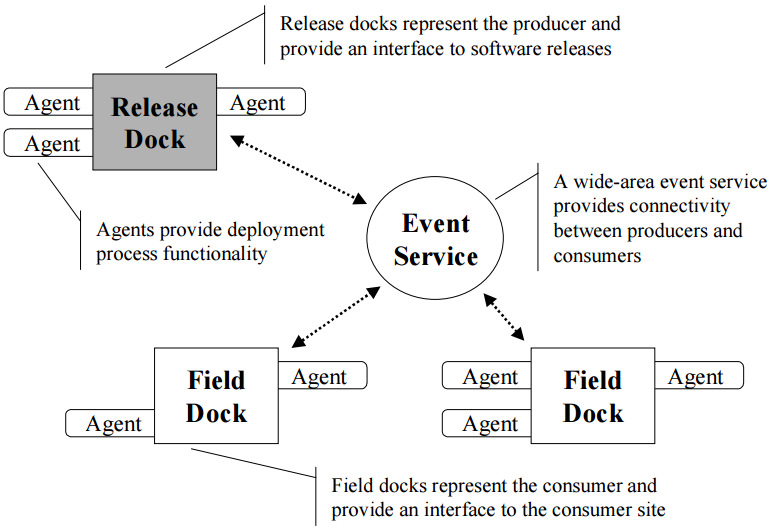
\includegraphics[scale=0.5]{afbeelding/softwareDockArchitectuur.png}}
%\caption{Software Dock Architectuur \citep{hall1999cooperative}}
%\label{fig:softwareDock}
%\end{figure}
%
%De release dock is een server die zich bevindt bij de software producent.
%Dit dock biedt een release repository aan waar de verbruikers de nodige software selecteren voor deployment.
%In de release dock wordt ieder release semantisch beschreven aan de hand van een Deployable Software Description file.
%Elke release wordt vergezeld door enkele agents die de semantische betekenis lezen en zo de deployment kunnen uitvoeren.
%Aan de hand van interfaces kunnen de agents aan de services en inhoud van de release dock.
%Bij het wijzigen van een software release zal de release dock verschillende events afvuren.
%Agents kunnen zich subscriben bij deze events en weten zo wanneer bepaalde handelingen uitgevoerd moeten worden \citep{hall1999cooperative}.
%
%De field dock dient als een interface naar de verbruiker kant toe.
%Deze interface biedt informatie over de resources en configuratie van het verbruiker systeem.
%Op basis van deze informatie wordt een context opgebouwd waarin de releases van de resource dock worden gedeployed.
%De agents die horen bij een release, docken zichzelf in de field dock en kunnen aan de hand van deze interface het verbruikers systeem ondervragen.
%Aangezien kritische client-side informatie op een gestandaardiseerde wijze aangeboden wordt, met behulp van een geneste collectie van pair-values die een hiërarchie vormen, kan de installatie van de software gepersonaliseerd worden \citep{hall1999cooperative}.
%
%\subsection{Case studies}
%Door de jaren heen zijn er verschillende technologieën ontwikkeld die het probleem van software deployment aanpakken.
%In wat volgt, worden enkele van deze technologieën besproken gebaseerd op enkele case studies die \citet{softwareDeployment} aanreikt.
%
%\subsubsection{Java Beans}
%Enterprise JavaBeans (EJB) zijn een standaard voor het bouwen van server-side componenten.
%De EJB's zijn speciaal ontworpen voor het vereenvoudigen van de deployment.
%\citet{softwareDeployment} beschrijft JavaBeans als eenheden van business logic in een component die uitgevoerd wordt in een container.
%De verschillende containers zorgen voor een abstractie van de hosting omgeving en bieden verscheidene services aan.
%Een JavaBean moet ingepakt worden volgens de specificaties die Sun Microsystems oplegt.
%Met deze standaard is het mogelijk om verschillende management en deployment tools te schrijven die de EJB's kunnen beïnvloeden.
%Enterprise JavaBeans worden ingepakt in de standaard Java JAR file, samen met een XML deployement descriptor.
%De descriptor beschrijft de verschillende eigenschappen van de bijhorende EJB.
%
%De Enterprise JavaBeans zijn volgens \citet{softwareDeployment} fijnkorrelige en taalafhankelijke oplossing voor het deployment probleem.
%Door het isoleren van de Beans door middel van een gestandaardiseerde container interface zullen Enterprise JavaBeans zo een oplossing vinden voor het deployment probleem.
%Hierdoor moeten de EJB's zodanig ontworpen worden dat ze voldoen aan de eisen van de interface.
%Enterprise JavaBeans hebben geen idee van het op afstand installeren van componenten.
%Een groot probleem bij EJB's is dat referenties naar afhankelijke beans gebeurd via niet unieke namen.
%Twee verschillende beans met eenzelfde naam moeten hierdoor manueel herladen worden zodanig dat de bindings up-to-date zijn \citep{rutherford2002reconfiguration}.
%
%\subsubsection{Redhat package manager}
%In Linux wordt de Redhat package manager (RPM) het vaakst gebruikt voor de deployment van software.
%Met hulp van de RPM is het mogelijk om enkele operaties uit te voeren zoals onder andere installatie, updaten, \ldots .
%De operaties worden ondersteund door een databank die alle informatie en details van de geïnstalleerde pakketten bevat.
%Een RPM pakket bestaat uit executables gecombineerd met configuratie bestanden en documentatie.
%Doordat een pakket executables bevat, zal een pakket gekoppeld zijn aan het besturingssysteem van de host \citep{bailey1997maximum}.
%Naast de RPM files bevat een pakket verschillende scripts geschreven in de standaard Unix scripting taal.
%De verscheidene scripts zijn ingedeeld in sets horende bij een specifieke taak.
%Bij een error moet een roll back uitgevoerd worden.
%Dit is de taak van de script schrijver \citep{softwareDeployment}.
%
%De Redhat Package Manager is in tegenstelling met de EJB's een grofkorrelige, taal onafhankelijke maar besturingssysteem afhankelijke oplossing.
%Het grootste probleem van RPM schuilt in de afhankelijkheden tussen de pakketten.
%Niet alle afhankelijkheden zijn explicite gemodelleerd en de afhankelijkheden die wel gemodelleerd zijn, zijn gevormd met de nadruk op de inhoud en niet op de pakketten zelf \citep{softwareDeployment}.  
%
%\subsubsection{ATLAS}\label{sec:ATLAS}
%Om in de ATLAS samenwerking om te gaan met de grote hoeveelheid bronnen, is er een volledig automatisch installatie systeem ontworpen voor het LCG/EGEE project, LHC Computing Grid/Enabling Grids for E-sciencE \citep{bird2005lhc}. 
%\citet{salvo2008atlas} beschrijft de architectuur van het ontworpen systeem.
%Het ontwerp van het installatie systeem werd gebaseerd op het Light Job Submission Framework for installation, ook wel LJSFi.
%
%\begin{figure}[!ht]
%\centering
%\makebox[0pt]{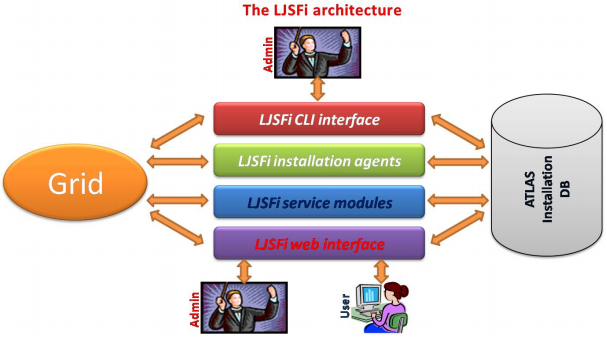
\includegraphics[scale=0.7]{afbeelding/ljsfiArchitectuur.png}}
%\caption{LJSFi Architectuur \citep{salvo2008atlas}}
%\label{fig:ljsfiArchi}
%\end{figure}
%
%De architectuur van het framework is zichtbaar in Figuur~\vref{fig:ljsfiArchi}.
%Het framework vormt een dunne laag over de middleware van Grid.
%De kern van het systeem bestaat uit de installatie database en de command line interface (CLI).
%De laatste zorgt voor de interacties met de Grid middleware.
%Met hulp van de installatie database kan de CLI verschillende taken en job informatie opslaan.
%Aan de hand van deze informatie kunnen installaties uitgevoerd worden.
%De installatie databank staat in contact met alle componenten van het framework.
%Zo kan de status van verscheidene acties en configuraties van verschillende taken opgeslagen worden.
%
%Naast deze twee grote componenten bevat LJSFi modules en extensies waarmee installatie aanvragen afgehandeld worden.
%Het systeem bevat drie verschillende componenten:
%\begin{itemize}
%\item \textbf{RAI module} De Request An Installation module dient als web interface voor het ontvangen van user-driven installatie aanvragen.
%\item \textbf{AIR module} De Automatic Installation Requester schiet in actie als software release aangeduid staan als productie of auto-installatie.
%De module verwijdert of installeert de software op alle sites waar de software nog niet gepubliceerd is.
%Door de AIR module periodiek te gebruiken, zullen de nodige aanvragen snel afgehandeld worden.
%\item \textbf{InAgent module} Met de InAgent module wordt het mogelijk om volledig geautomatiseerde installatieprocessen te voorzien.
%Iedere 10 minuten wordt de Installation database gelezen en via de CLI interface worden de nodige installatieprocessen opgestart.
%Elk installatieproces wordt bijgestaan door een installation agent.
%De agent zal instaan voor het updaten van de Installatie database met real-time informatie die zichtbaar is online.
%\end{itemize}
%
%Naast de verscheidene automatische services biedt LJSFi enkele gebruiker services aan.
%Een gebruiker kan zich subscriben voor bepaalde acties op een doel systeem.
%Als deze actie wordt uitgevoerd dan krijgt de gebruiker een mail.
%Hiernaast kan een gebruiker een software release vastpinnen zodat deze niet verwijderd kan worden door het systeem.
%
%Het installatieproces wordt uitgevoerd in drie verschillende stappen.
%In een eerste stap wordt een site check uitgevoerd door een pilot job naar de site te sturen.
%Als de check succesvol uitgevoerd wordt, kan het installatieproces beginnen.
%De acties tijdens het installatieproces worden uitgevoerd door softwaremanagement scripts.
%Op het einde van het proces, haalt het systeem de job output en exit code op.
%De laatste wordt opgeslagen in de Installation database.
%
%\subsubsection{ORYA}\label{sec:ORYA}
%\citet{lestideau2003providing} legt uit hoe met ORYA (Open enviRonment to deploY Applications) verschillende deployment functionaliteiten aanbiedt aan gedistribueerde, autonome entiteiten zoals workstations en servers.
%Aan de hand van een deployment PSEE \citep{belkhatir2007adele} wordt het mogelijk om het installatieproces te automatiseren.
%
%In het ontwerp van ORYA worden er drie verschillende entiteiten besproken die nodig zijn om het automatische installatieproces mogelijk te maken.
%\begin{itemize}
%\item \textbf{Applicatie Server} De applicatie server bevat nodige informatie nodig voor de installatie.
%Hieronder bevindt zich onder andere een pakket met de nodige resources en een manifest waarin de afhankelijkheden, beperkingen en features staan.
%\item \textbf{Target} De target is het doel waarop de deployment uitgevoerd wordt.
%Iedere target wordt beschreven door de verschillende applicaties die al aanwezig zijn en de fysische beschrijving.
%\item \textbf{Deployment Server} De deployment server vormt de kern van de deployment omgeving en staat in voor het uitvoeren van de deployments. 
%De deployment server zoekt de nodige pakketten, voert een transfer van de pakketten uit en installeert de applicatie.
%Op het einde moet de deployment server garanderen dat vorige programma's correct blijven functioneren.
%\end{itemize}
%
%\citet{lestideau2003providing} beschrijft verder de verschillende modellen die gehanteerd worden om een succesvolle deployment uit te voeren.
%In Figuur~\vref{fig:deploymentModel} is het deployment proces model terug te vinden.
%Een deployment proces zal bestaan uit verschillende basis activiteiten en deployment processen.
%Iedere activiteit wordt uitgevoerd door een agent.
%
%\begin{figure}[!ht]
%\centering
%\makebox[0pt]{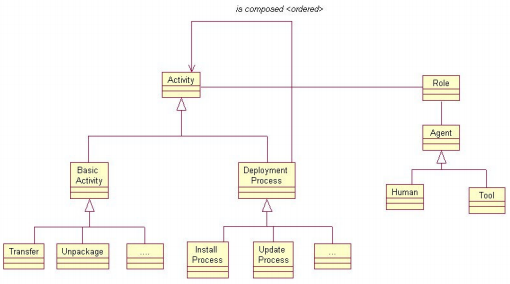
\includegraphics[scale=0.7]{afbeelding/deploymentModelORYA.png}}
%\caption{Deployment proces model \citep{lestideau2003providing}}
%\label{fig:deploymentModel}
%\end{figure}
%
%Een toegepast voorbeeld van een deployment aan de hand van dit model is terug te vinden in Figuur~\vref{fig:deploymentVoorbeeld}.
%Een basis activiteit wordt voorgesteld aan de hand van een grijze rechthoek en een deployment proces aan de hand van een witte rechthoek.
%In het voorbeeld zijn dus vier deployment processen aanwezig en 3 basis activiteiten.
%
%\begin{figure}[!ht]
%\centering
%\makebox[0pt]{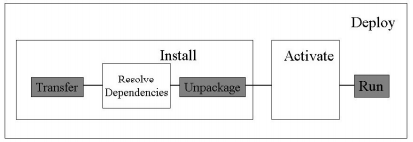
\includegraphics[scale=0.7]{afbeelding/deploymentVoorbeeld.png}}
%\caption{Voorbeeld van een deployment \citep{lestideau2003providing}}
%\label{fig:deploymentVoorbeeld}
%\end{figure}
%
%Aan de hand van deze structuur wordt het mogelijk om het volledige deployment proces voor te stellen.
%
%\subsubsection{Nix}
%\citet{dolstra2006purely} bespreekt hoe Nix systemen omgaan met het deployment probleem.
%Nix houdt verschillende componenten bij in de component store waarbij iedere component een set van bestanden is.
%De componenten worden van elkaar gescheiden door een unieke naam.
%Dit wordt bekomen door een cryptografische hash op te nemen in de naam.
%Nix biedt geen software deployment aan.
%Het biedt verscheidene mechanismen aan waarmee verschillende deployment beleid beschikbaar worden.
%Met de volgende deployment models is het mogelijk om in Nix de Nix expressies (de bouwstenen van de Nix componenten) te verspreiden:
%\begin{itemize}
%\item \textbf{Handmatige download} Een gebruiker kan zelf pakketten downloaden in de vorm van tar archieven, deze zelf uitpakken en vervolgens installeren.
%Deze strategie is arbeidsintensief en maakt het moeilijk om alles up-to-date te houden. 
%\item \textbf{Updaten aan de hand van een versie management systeem} Een andere strategie is het gebruik van een versie management systeem.
%Hiermee is het up-to-date houden van de pakketten zeer eenvoudig.
%\item \textbf{Kanalen} Een verdere uitbreiding zijn de kanalen.
%Een kanaal is een URL naar een tar archief die de nodige Nix expressies bevat.
%Met deze strategie is het even eenvoudig om pakketten te installeren en up-to-date te houden.
%\item \textbf{One-click installatie} Als er enkel één pakket geïnstalleerd moet worden, dan is de one-click installatie de eenvoudigste optie.
%Via de website van de verdeler kan een link gebruikt worden om het nodige pakket te installeren.
%\end{itemize}

\section{Deployment environment}
%%% TODO uitbreiden met de verschillende nieuwe bronnen die er ook over praten
%\subsection{Software levenscyclus}\label{sec:softwareLevenscyclus}
%De levenscyclus van software deployment kan volgens \citet{softwareDeployment,hall1999cooperative} beschreven worden in verschillend stappen, namelijk:
%\begin{itemize}
%\item \emph{Release}: de software is volledig samengesteld uit pakketten die voldoende metadata bevatten om de verschillende bronnen te beschrijven waarvan het pakket afhangt.
%\item \emph{Installatie}: de software moet overgebracht worden naar de client en geconfigureerd worden in voorbereiding op de activatie.
%\item \emph{Activeren}: tijdens de activatie wordt de software uitvoering opgestart of worden de nodige triggers geplaatst om de executie op het gepaste tijdstip op te starten.
%\item \emph{Deactiveren}: dit is tegengesteld aan activeren. Deze stap is voor nodig voordat een aanpassing of herconfiguratie kan uitgevoerd worden.
%\item \emph{Updaten}: dit is het proces waarin de software wordt aangepast. Deze stap wordt vaak geactiveerd door het uitbrengen van een nieuwe versie van de software.
%\item \emph{Deïnstallatie}: tijdens deze stap zal de geïnstalleerd software van het client systeem gehaald worden.
%\end{itemize}
%De enige fase van de levenscyclus die zich uitsluitend op de server afgespeeld is de release fase.
%De rest van de fases spelen zich af op de verschillende client systemen.
%
%\begin{figure}[!ht]
%\centering
%\makebox[0pt]{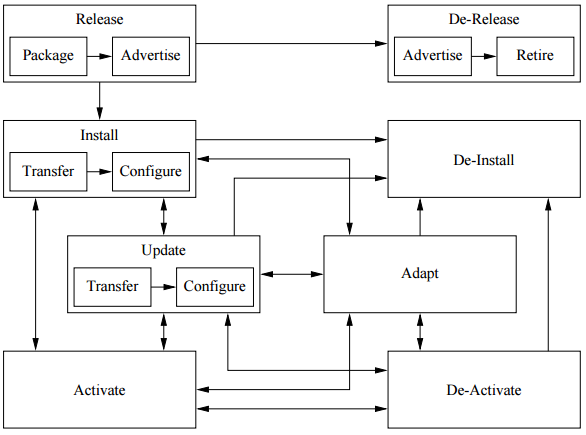
\includegraphics[scale=0.7]{afbeelding/softwareLevenscyclus.png}}
%\caption{Levenscyclus van software \citep{carzaniga1998characterization}}
%\label{fig:softwareLevenscyclus}
%\end{figure}
%
%%%% TODO schrijven over de problemen die komen bij het deployen
%In theorie zou het deployen van software een eenvoudig probleem moeten zijn.
%Aangezien software bestaat uit een set van bestanden, dan zou het deployen van software naar een doelcomputer slechts bestaat uit het kopiëren van de nodige bestanden.
%Maar dit is vaak niet het geval.
%Volgens \citet{dolstra2006purely} zijn er in de praktijk verschillende oorzaken die ervoor zorgen dat het deployment probleem ingewikkelder wordt.
%Deze oorzaken kunnen in twee grote categorieën ingedeeld worden, namelijk de omgevings- en de onderhoudsproblemen.
%
%\paragraph{Omgevingsproblemen}
%In de eerste categorie ligt de nadruk vooral op correctheid.
%Voordat de software geïnstalleerd wordt op een doelsysteem, wordt de doelomgeving ondervraagt naar alle eigenschappen: zijn de nodige programma's aanwezig, bestaan alle configuratie bestanden, \ldots .
%Als deze eisen niet voldaan zijn, dan zal de software niet werken zoals gewenst.
%\citet{dolstra2006purely} haalt enkele concrete voorbeelden aan van omgevingsproblemen:
%\begin{itemize}
%\item De deployment van software kan een gedistribueerd probleem zijn.
%Software kan afhankelijk zijn van componenten draaiende op verwijderde systemen of van andere processen draaiende op het doelsysteem.  
%\item Software is vaak afhankelijk van verschillende andere software componenten. 
%Deze afhankelijkheden, of ook wel dependencies genoemd, moeten voor de deployment bepaald worden.
%Dit proces is moeilijk en een fout kan pas laat ontdekt worden.
%\item De dependencies moeten compatibel zijn met wat er verwacht wordt van de software.
%Niet elke versie zal werken.
%Sommige depencies vertonen build-time variaties.
%De component kan dan gebouwd zijn met enkele optionele eigenschappen of eigenschappen die gekozen worden at build-time.
%\item Sommige software componenten zijn afhankelijk van specifieke hardware.
%Dit kan enkel verholpen worden door op voorhand te controleren welke hardware aanwezig is.
%\end{itemize}
%Uit deze concrete voorbeelden wordt het snel duidelijk dat er twee problemen zijn: de verschillende eisen van de software moeten geïdentificeerd worden en vervolgens moeten deze gerealiseerd worden in het doelsysteem.
%
%\paragraph{Onderhoudsproblemen}
%Naast de verschillende omgevingsproblemen, beschrijft \citet{dolstra2006purely} ook enkele onderhoudsproblemen.
%Software moet kunnen ``evolueren''.
%Om dit te ondersteunen, moeten allerlei actie zoals upgraden en updaten uitvoerbaar zijn.
%Enkele voorbeelden van zulke acties zijn:
%\begin{itemize}
%\item Tijdens het verwijderen van software, moeten alle componenten verwijderd worden.
%Ondertussen mogen geen componenten verwijderd worden die nog in gebruik zijn door andere software.
%\item Ook tijdens het updaten van software moet rekening gehouden worden met andere software.
%Het updaten van een component kan voor problemen en failure zorgen in een andere component.
%Een DLL-hell wordt best ten alle tijden vermeden.
%\item Na het upgraden/updaten van een component, is het soms aangewezen om een roll back uit te voeren.
%Zo'n actie kan overwogen worden als de upgrade belangrijke functionaliteiten van de software kapot maakt.
%\end{itemize}
%
%\subsection{Rollback}
%Het deployen van software op een doelsysteem brengt verscheidene problemen met zich mee.
%Bij het voorkomen van een probleem moet een mechanisme aanwezig zijn zodanig dat de problemen opgevangen worden.
%
%\subsubsection{Rollback strategieën}
%%%% TODO
%Stuk schrijven over rollback strategieën? Kan dan eenvoud vm aanhalen?
%\citet{srinivasan2004flashback} bespreekt 3 mogelijke manieren van rollback
%\citet{elnozahy2002survey} $->$ is vooral voor gedistribueerde systemen (is dit wel van toepassing hier?)
%\citet{machado2008enabling} $->$ rollback maar dan atomisch
%
%%%% VRAAG wat doen als configuratie file compromised is?
%
%\subsubsection{Virtualisatie}\label{sec:virtualisatie}
%\citet{softwareDeployment} brengt virtualisatie ter sprake.
%Door middel van virtualisatie wordt de complexiteit die ontstaat door de interactie tussen het programma, de installatieomgeving en de uitvoeringsbeperkingen gelimiteerd.
%Door het creëren van een perfecte omgeving komen deze problemen niet voor.
%Er zijn verschillende voordelen gekoppeld aan het gebruiken van een virtuele machine.
%Bijvoorbeeld, besturingssystemen op verschillende hardware platformen eisen verschillende drivers en deze drivers hebben misschien afhankelijkheden op een bepaalde firmware en BIOS.
%Een guest OS draaiende op een virtuele machine heeft deze eisen niet \citep{shumate2004implications}.
%
%
%%%% TODO
%De structuur die \citet{shumate2004implications} voorstelt voor het deployen van VM images lijkt handig
%
%
%Maar virtualisatie is niet de enige techniek die gebruikt zou kunnen worden om rollbacks te vermijden.
%Docker containers is een technologie waarmee een stuk software wordt ingepakt in een volledig filesysteem dat alle benodigdheden bevat om correct te functioneren.
%Hierdoor zal de software overal op eenzelfde manier draaien, ongeacht de omgeving \citep{dockerMain}.
%Docker containers is niet hetzelfde als virtuele machines.
%\citet{dockerEbook} bespreekt de twee aan de hand van een vergelijking.
%In de vergelijking worden virtuele machines voorgesteld als huizen terwijl Docker containers worden voorgesteld als appartementen.
%
%De huizen staan volledig op zichzelf en bieden bescherming tegen ongewenste gasten.
%Ze hebben een eigen infrastructuur met hun eigen water, verwarming, \ldots .
%Hiernaast zal ieder huis op zijn minste een badkamer, living, slaapkamer en keuken hebben.
%Het vinden van een klein huis is een ganse klus en vaak zal een huis meer bevatten dan nodig is want dat komt door de manier waarop huizen gebouwd worden.
%
%Appartementen bieden ook bescherming tegen ongewenste gasten, maar zij zijn gebouwd rond een gemeenschappelijke infrastructuur.
%Het appartementsgebouw biedt gemeenschappelijk water, verwarming, \ldots  aan, aan elk appartement.
%Elk appartement verschilt ook nog van grootte.
%Er bestaan kleine appartementen maar ook grote met meerder slaapkamers.
%Men huurt enkel hetgeen dat nodig is.
%
%\begin{figure}[!ht]
%\centering
%\makebox[0pt]{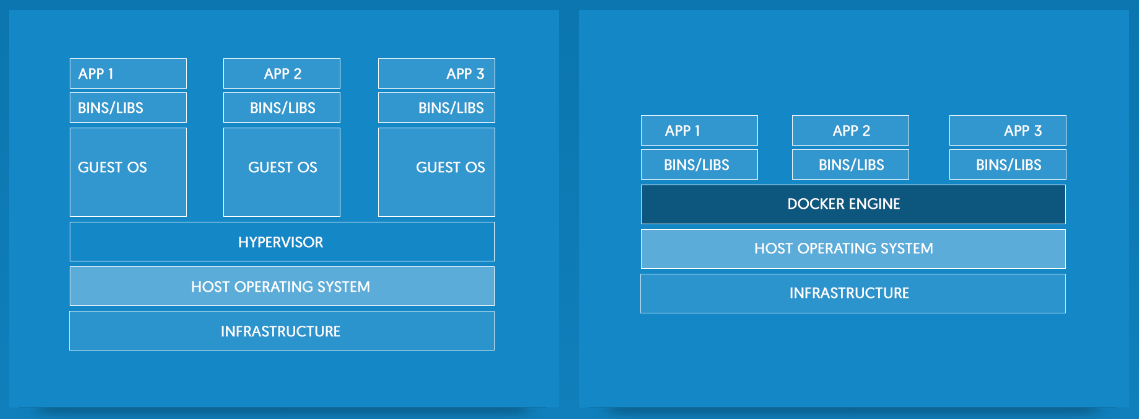
\includegraphics[scale=0.5]{afbeelding/dockerVsVM.png}}
%\caption{Architectuur van Virtuele Machine ten opzichte van Docker \citep{dockerMain}}
%\label{fig:VMvsDocker}
%\end{figure}
%
%In Figuur~\vref{fig:VMvsDocker} zijn de architecturen van virtuele machines en Docker terug te vinden.
%Het verschil tussen beiden wordt al snel duidelijk.
%Een virtuele machine zal typisch de applicatie, de nodige binaries en bibliotheken en een volledig besturingssysteem bevatten.
%Een container bevat de applicatie en de verschillende dependencies maar de kernel wordt gedeeld met alle andere containers en gedragen zich als een geïsoleerd proces in de user space van het host besturingssysteem.
%
%\citet{chamberlain2014using} bespreekt kort hoe Docker werkt.
%Docker is een platform dat gebruik maakt van de Linux Containers (LXC de user-space control package voor Linux Containers) om software te encapsuleren.
%LXC is een virtualisatie techniek waarmee virtuele omgevingen in Linux opgebouwd kunnen worden.
%De containers zullen processen van elkaar sandboxen zodanig dat een proces een ander niet kan beïnvloeden \citep{merkel2014docker}.
%Docker zal de LXC software uitbreiden waardoor deployment, distributie en versioning mogelijk wordt.
%Naast LXC gebruikt Docker AuFS (Advanced Multi-Layered Unification Filesystem) als het filesysteem voor de containers.
%Doordat het filesysteem gelaagd is, is het mogelijk om verschillende filesystemen over elkaar te leggen.
%
%\citet{merkel2014docker} vergelijkt de twee virtualisatie technieken en bespreekt de verschillende tussen de twee.
%Bij virtuele machines moet voor iedere virtuele machine een besturingssysteem geïnstalleerd worden.
%Al deze besturingssystemen verbruiken RAM, CPU en bandbreedte.
%Containers zullen piggybacken op het bestaande host besturingssysteem.
%Hierdoor zal het resource gebruik efficiënter zijn.
%Een container is goedkoop waardoor het creëren en verwijderen van containers een snelle operatie.
%Dit komt omdat er enkel een proces moet afgesloten worden in tegenstelling tot het afsluiten van een volledig besturingssysteem.
%Een voordeel van de VMs ten opzichte van Docker is hun maturiteit.
%VMs bestaan langer en hebben zichzelf kunnen bewijzen in verschillende situaties.
%
%%%% TODO zeggen dat docker wel de beste oplossing is voor roll back te omzeilen